\id{МРНТИ 06.56.31}{https://doi.org/10.58805/kazutb.v.2.27-927}

\begin{articleheader}
\sectionwithauthors{M.T. Zhumazhanova, B.S.Saparova, Syed Faisal Hassan Bukhari}{MODELS AND CONCESSIONS FOR THE DEVELOPMENT OF PUBLIC-PRIVATE PARTNERSHIP IN KAZAKHSTAN IN THE CONTEXT OF DIGITALIZATION}

{\bfseries
\textsuperscript{1}M.T. Zhumazhanova\alink{https://orcid.org/0009-0008-0413-9057}\textsuperscript{\envelope },
\textsuperscript{2}B.S.Saparova\alink{https://orcid.org/0000-0002-0881-3474},
\textsuperscript{3}Syed Faisal Hassan Bukhari\alink{https://orcid.org/0000-0002-6971-1498}
}
\end{articleheader}

\begin{affiliation}
\textsuperscript{1}Kazakh University of Technology and Business named after K.Kulazhanov, Astana, Kazakhstan,

\textsuperscript{2}"L.N.Gumilyov Eurasian National University" Astana, Kazakhstan,

\textsuperscript{3}Air University, Islamabad, Pakistan

\raggedright \textsuperscript{\envelope }Corresponding author: maral2804@mail.ru
\end{affiliation}

The scientific article analyzes the development of public-private
partnership (PPP) in Kazakhstan, models and development concessions in
the context of digitalization. As part of the economic transformation,
PPP is becoming an important tool for diversifying the economy,
modernizing infrastructure, and improving the quality of public
services. The key areas of effective cooperation between the state and
the private sector are considered, as well as the main problems,
including insufficient institutional maturity, risks, corruption threats
and the uncertainty of the political situation. Special attention is
paid to attracting investments, innovative technologies and experience
for the successful implementation of PPP projects.

The success of PPP in Kazakhstan depends on the creation of a stable
institutional framework, ensuring transparency and improving the skills
of government agencies. One of the priorities is the digitalization of
the PPP system, which helps to improve project management, increase
transparency and reduce the risks of corruption. The article provides
examples of successful digital solutions such as electronic tender
platforms and monitoring systems that have improved the interaction
between public and private institutions.

Digitalization is an important factor in increasing the efficiency and
sustainability of the PPP system in Kazakhstan. To fully unlock its
potential, it is necessary to solve existing problems such as
insufficient infrastructure and standards for digital solutions, as well
as create platforms for effective data exchange and project monitoring.
In the context of digitalization, PPP models such as concessions and
public-private partnerships can be adapted to introduce innovative
technologies, which will accelerate the implementation of infrastructure
projects and ensure their long-term sustainability by ensuring
cooperation between public and private interests.

{\bfseries Keywords:} public-private partnership, concession, models,
innovations, messages, GDP, digital technologies, Public-private
agreements, infrastructure projects, digitalization, modernization.

\begin{articleheader}
{\bfseries ЦИФРЛАНДЫРУ ЖАҒДАЙЫНДА ҚАЗАҚСТАННЫҢ МЕМЛЕКЕТТІК-ЖЕКЕШЕЛІК ӘРІПТЕСТІГІН ДАМЫТУ МОДЕЛЬДЕРІ МЕН КОНЦЕССИЯЛАРЫ}

{\bfseries
\textsuperscript{1}М. Т.Жұмажанова\textsuperscript{\envelope },
\textsuperscript{2}Б.С.Сапарова,
\textsuperscript{3}Syed Faisal Hassan Bukhari
}
\end{articleheader}

\begin{affiliation}
\textsuperscript{1 «}Қ. Құлажанов атындағы Қазақ технология және бизнес университеті» АҚ., Астана, Қазақстан,

\textsuperscript{2}"Л.Н. Гумилев атындағы Еуразия ұлттық университеті" Астана, Қазақстан,

\textsuperscript{3}«Әуе университеті», Исламабад, Пәкістан

e-mail: maral2804@mail.ru
\end{affiliation}

Ғылыми мақалада Қазақстандағы мемлекеттік-жекешелік әріптестіктің (МЖӘ)
дамуы, цифрландыру жағдайындағы даму модельдері мен концессиялары
талданады. Экономикалық трансформация шеңберінде МЖӘ экономиканы
әртараптандыру, инфрақұрылымды жаңғырту және мемлекеттік көрсетілетін
қызметтердің сапасын арттыру үшін маңызды құралға айналады. Мемлекет пен
жеке сектордың тиімді ынтымақтастығының негізгі бағыттары, сондай-ақ
институционалдық жетілудің жеткіліксіздігін, тәуекелдерді, сыбайлас
жемқорлық қатерлерін және саяси ахуалдың белгісіздігін қоса алғанда,
негізгі проблемалар қаралады. МЖӘ жобаларын табысты іске асыру үшін
инвестицияларды, инновациялық технологияларды және тәжірибені тартуға
ерекше назар аударылды.

Қазақстандағы МЖӘ табысы тұрақты институционалдық базаны құруға,
ашықтықты қамтамасыз етуге және мемлекеттік органдардың біліктілігін
арттыруға байланысты. Жобаларды басқаруды жақсартуға, ашықтықты
арттыруға және сыбайлас жемқорлық тәуекелдерін азайтуға ықпал ететін МЖӘ
жүйесін цифрландыру басым бағыттардың бірі болып табылады. Мақалада
мемлекеттік және жеке мекемелер арасындағы өзара әрекеттесуді жақсартқан
электронды тендерлік платформалар мен бақылау жүйелері сияқты сәтті
цифрлық шешімдердің мысалдары келтірілген.

Цифрландыру Қазақстандағы МЖӘ жүйесінің тиімділігі мен тұрақтылығын
арттырудың маңызды факторы болып табылады. Оның әлеуетін толық ашу үшін
инфрақұрылымның жеткіліксіздігі және цифрлық шешімдер стандарттары
сияқты бар мәселелерді шешу, сондай-ақ деректерді тиімді бөлісу және
жобаларды бақылау үшін платформалар құру қажет. Цифрландыру жағдайында
концессиялар мен мемлекеттік-жекешелік әріптестіктер сияқты МЖӘ
модельдері инновациялық технологияларды енгізуге бейімделуі мүмкін, бұл
инфрақұрылымдық жобаларды іске асыруды жеделдетуге және мемлекеттік және
жеке мүдделер арасындағы ынтымақтастықты қамтамасыз ете отырып, олардың
ұзақ мерзімді орнықтылығын қамтамасыз етуге мүмкіндік береді.

{\bfseries Түйін сөздер:} мемлекеттік-жекешелік әріптестік, концессия,
модельдер, инновациялар, Жолдаулар, ЖІӨ, цифрлық технологиялар,
Жария-жекешелік келісімдер, инфрақұрылымдық жобалар, цифрландыру,
жаңғырту.

\begin{articleheader}
{\bfseries МОДЕЛИ И КОНЦЕССИИ РАЗВИТИЯ ГОСУДАРСТВЕННО-ЧАСТНОГО ПАРТНЕРСТВА КАЗАХСТАНА В УСЛОВИЯХ ЦИФРОВИЗАЦИИ}

{\bfseries
\textsuperscript{1}М.Т.Жумажанова\textsuperscript{\envelope },
\textsuperscript{2}Б.С.Сапарова.,
\textsuperscript{3}Syed Faisal Hassan Bukhari
}
\end{articleheader}

\begin{articleheader}
\textsuperscript{1}Казахский университет технологии и бизнеса им.К.Кулажанова, Астана, Казахстан,

\textsuperscript{2}Евразийский национальный университет им. Л.Н.Гумилева, Астана, Казахстан,

\textsuperscript{3}Воздушный университет, Исламабад, Пакистан,

e-mail: maral2804@mail.ru
\end{articleheader}

В научной статье анализируется развитие государственно-частного
партнерства (ГЧП) в Казахстане, модели и концессии развития в условиях
цифровизации. В рамках экономической трансформации ГЧП становится важным
инструментом для диверсификации экономики, модернизации инфраструктуры и
повышения качества государственных услуг. Рассматриваются ключевые
направления эффективного сотрудничества государства и частного сектора,
а также основные проблемы, включая недостаточную институциональную
зрелость, риски, коррупционные угрозы и неопределенность политической
ситуации. Особое внимание уделено привлечению инвестиций, инновационных
технологий и опыта для успешной реализации проектов ГЧП.

Успех ГЧП в Казахстане зависит от создания устойчивой институциональной
базы, обеспечения прозрачности и повышения квалификации государственных
органов. Одним из приоритетных направлений является цифровизация системы
ГЧП, которая способствует улучшению управления проектами, повышению
прозрачности и снижению рисков коррупции. В статье приведены примеры
успешных цифровых решений, таких как электронные платформы для тендеров
и системы мониторинга, которые улучшили взаимодействие между
государственными и частными учреждениями.

Цифровизация является важным фактором повышения эффективности и
устойчивости системы ГЧП в Казахстане. Для полного раскрытия ее
потенциала необходимо решить существующие проблемы, такие как
недостаточная инфраструктура и стандарты цифровых решений, а также
создать платформы для эффективного обмена данными и мониторинга
проектов. В условиях цифровизации модели ГЧП, такие как концессии и
публично-частные партнерства, могут быть адаптированы для внедрения
инновационных технологий, что позволит ускорить реализацию
инфраструктурных проектов и обеспечить их долгосрочную устойчивость,
обеспечивая сотрудничество между государственными и частными интересами.

{\bfseries Ключевые слова}: государственно-частное партнерство, концессия,
модели, инновации, послания, ВВП, цифровые технологии, Публично-частные
соглашения, инфраструктурные проекты, цифровизация, модернизация.

\begin{multicols}{2}
{\bfseries Introduction.} In the annual messages of the President of
Kazakhstan, namely from 2020-2024, special attention is paid to the
development of PPP as a key tool for modernizing infrastructure and the
social sphere. Kassym-Jomart Tokayev focuses on the importance of
creating a transparent and sustainable PPP system, which will improve
the quality of public services and attract significant private
investment, including foreign partners.

In the President' s Address to the People of Kazakhstan
"Kazakhstan in a new reality: Time for Action" in 2020, Kassym--Jomart
Kemeluly outlined the need to strengthen the role of PPP in the
country' s economy. The president noted that
entrepreneurship should be an active and key partner of the country in
solving social and infrastructure problems. In particular, Kassym-Jomart
Kemelovich noted that it is necessary to improve regulatory and
legislative acts on the implementation of PPP projects, optimize
procedures, processes and develop additional incentive programs for
private investors. Tokayev, in his address to the people of Kazakhstan
in 2021 with the title" Hadik unity and systemic reforms -- a solid
foundation for the country' s prosperity", once again
emphasized the relevance of public-private partnership as the main
mechanism for infrastructure and social modernization. He noted that it
is necessary to step up the participation of the private sector in
projects such as the construction of schools, hospitals and roads.

In the 2022 Message, "A just State. One nation. Prosperous Society"
Tokayev continued to focus on attracting private investment through PPP
in the development of infrastructure and housing and communal services.

In his 2023 Address "The Economic Course of a Just Kazakhstan," Tokayev
reiterated the importance of PPPs for the implementation of
infrastructure projects, as well as for attracting private investment in
the social sphere. In particular, he noted the need to increase the
number of successful PPP projects in the fields of healthcare, education
and housing construction.

In the 2024 Address "Fair Kazakhstan: Law and Order, economic growth,
public optimism", the President again pointed to the role of PPP as a
tool for infrastructure development and improving the quality of life of
the population. In this context, special attention was paid to
increasing the scale and coverage of PPP projects in new areas such as
ecology, digitalization and the development of "smart" cities {[}1{]}.

Present literature on PublicPrivate Partnership (PPPs) in Kazakhstan
mainly focuses on traditional frameworks and overlooking
digitalization' s role in enhancing concession models
{[}2{]}. The republic of Kazakhstan experiences digital
transformation,resultantlynew technologies like blockchain and AI offer
openings to improve PPP governance and efficiency {[}3{]}. However, a
more organized approach by integrating these technologies into PPPs is
still lacking and creating investment uncertainties. This research study
fills the gap by offering a digitalized PPP framework, assessing
governance mechanisms and providing policy recommendations. It also
empirically evaluates digitalization's impact on PPP performance, aiming
more transparent, efficient, and sustainable PPP environment in
Kazakhstan {[}4{]}.

 As part of the study of the role of PPP
in the development of Kazakhstan and the introduction of digital
technologies in this process, a multifaceted approach is used, including
quantitative, qualitative methods of analysis and SWOT analysis. To
achieve the set goals and on the way to the implementation of the tasks,
the following methods are proposed:

Study of legislative and normative documents;

Analysis of public-private partnership projects;

Analysis of statistical publications in the direction of PPP;

Comparison of Kazakhstan' S PPP process with
international experience;

Development of proposals for forecasting PPP improvements

Conducting a comprehensive analysis and reviewing reports.

The scientific article examines the current state of public-private
partnership in the Republic of Kazakhstan and analyzes it. In addition,
the prospects for the further development of the PPP industry using
digital technologies were considered. The article used various
literature, normative acts, articles and methodological approaches,
including the use of analytical tools, as well as forecasting models.
This approach makes it possible not only to understand current issues,
but also to develop specific recommendations for improving the
efficiency of PPPs through innovation and digitalization at all levels.

Kazakhstan is the largest landlocked country in the world, with one of
the lowest population densities in the world. It has a strategic
location in the center of the Eurasian continent at the crossroads of
the routes between the People' s Republic of China and
Western Europe, connected by road and rail transport and a port on the
Caspian Sea. The Republic of Kazakhstan is a medium-income and
economically dependent state on natural resources, including energy. But
despite this, our country is a developing state. Our country ranks 9th
in terms of oil reserves in the world, which, according to 2020,
accounted for 19.5\% of gross domestic product and 73\% of exports in
2023. In 2020, after the COVID -- 19 pandemic, Kazakhstan' s
GDP decreased by 2.5\%. This was the first time in 20 years. However, in
2021, the situation returned to normal and the volume of GDP was
recorded at 4.3\%. The Asian Development Bank estimates that GDP growth
in 2022 will be approximately 3.0\% as a result of increased domestic
activity, a recovery in global oil demand, ongoing fiscal support
measures and a successful vaccination program aimed at combating the
COVID pandemic.

In February 2021, Kazakhstan updated its National Development Plan until
2025, which sets out a medium-term vision for economic diversification
through reforms in the agro-industrial and transport sectors, support
for small and medium-sized enterprises, as well as the development of
tourism and other sectors. The main goal of this plan is to increase
liquidity, as well as increase the volume of private investment. This,
in turn, will help our state to become one of the 30 richest economies
by 2030. The Parliament of the Republic of Kazakhstan has completed the
development of a new economic policy "Adil Kazakhstan", approved in
September 2022.

The main principles of this policy are guaranteeing entrepreneurship,
creating a favorable investment climate in the country, increasing
activity, effective management of public finances, reducing
administrative barriers, minimizing the role of the state in the economy
and social protection of the population. Estimates show that annual
investment currently accounts for about 20\% of GDP, compared with an
average of 28\% in the richest 30 countries. Therefore, it is expected
that the Government' s consistent efforts will contribute
to creating more favorable conditions for private investment.

In the period from 1990 to 2020, 23 PPP projects of national importance
in various sectors such as transport (including roads, railways and
airports), energy, ICT and solid household waste (MSW) reached financial
closure. The total investment in these projects amounted to about 2.6
billion US dollars. During this period, one PPP project (the agreement
for the management of Astana Airport) was cancelled, which is 4\% of the
total number of projects. The energy sector was the most active,
accounting for 73\% of the total number of projects that reached
financial closure. Figure 1 shows the number of PPP projects that have
reached financial closure.

According to Figure 1, the largest number of financially closed projects
is in the energy sector.

The distribution of projects by industry is shown in the figure below.
(Fig.2)
\end{multicols}

\begin{figure}[H]
	\centering
	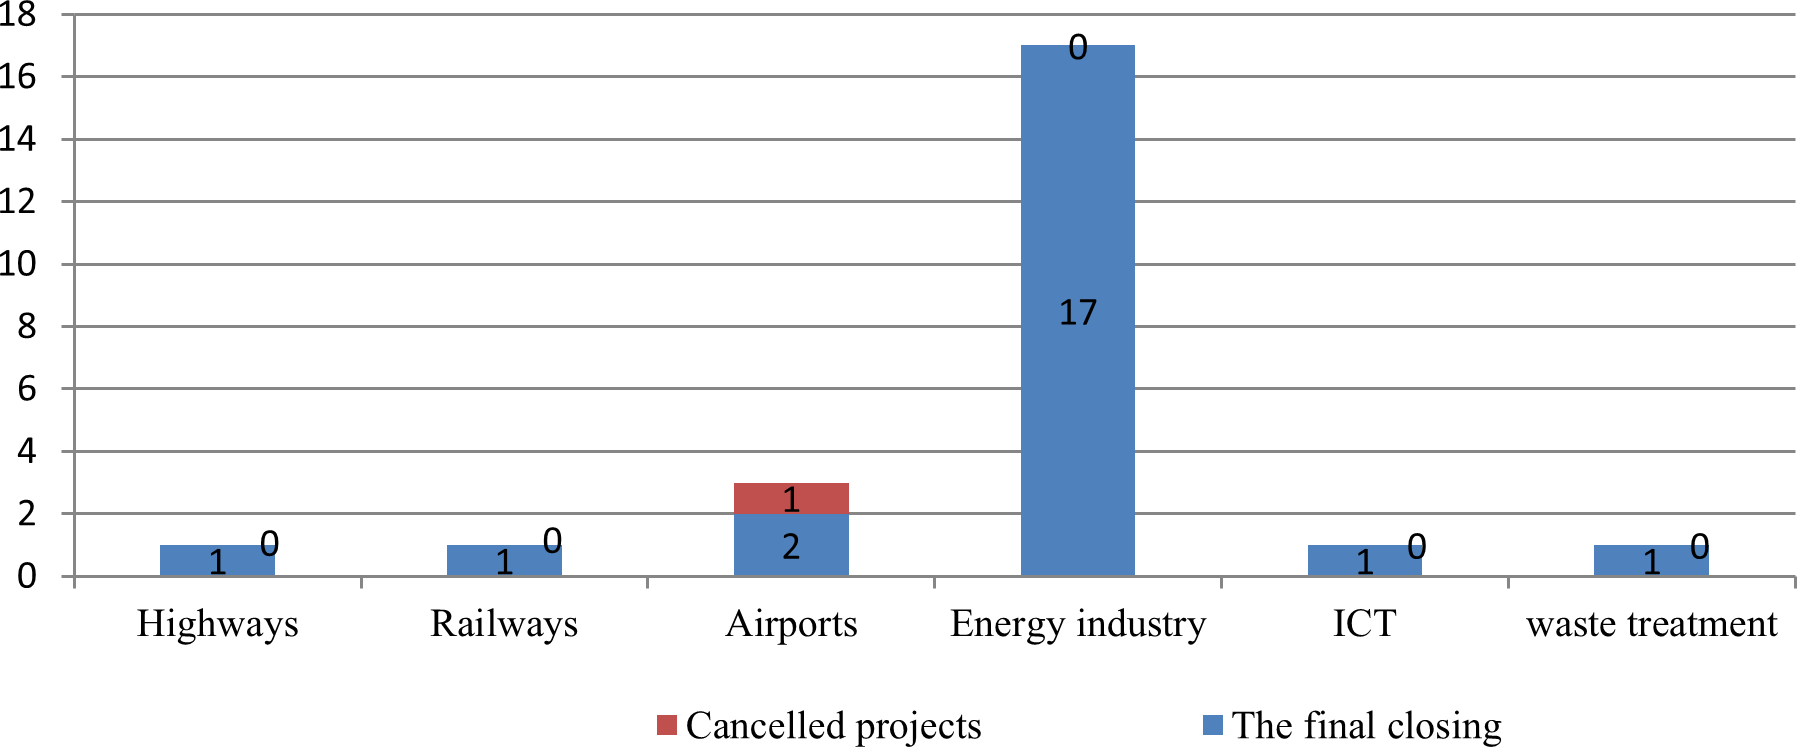
\includegraphics[width=0.7\textwidth]{media/ekon4/image17}
	\caption*{Fig.1 - PPP projects in Kazakhstan that reached financial closure and were cancelled in the period from independence to 2020}
	\caption*{\normalfont\emph{Note: compiled by the author based on Asiap development bank data:
"Overview of Public-Private Partnership in Kazakhstan" {[}5{]}}}
\end{figure}

\begin{figure}[H]
	\centering
	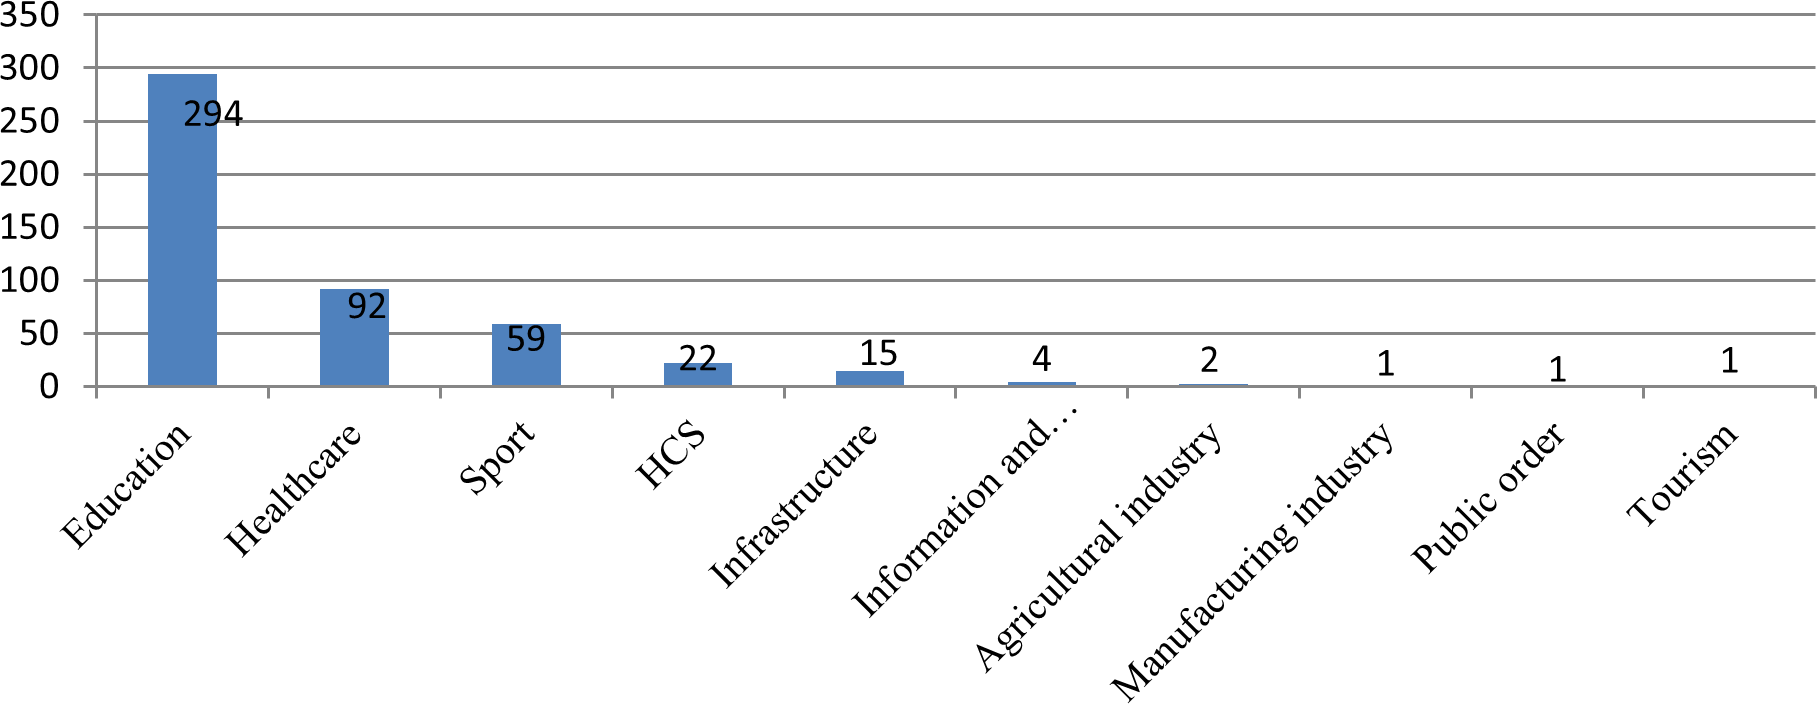
\includegraphics[width=0.7\textwidth]{media/ekon4/image18}
	\caption*{Fig.2 - Distribution of projects by industry}
	\caption*{\normalfont\emph{Note: Compiled by the author on the basis of data from JSC "Kazakhstan PPP Development Center" {[}6{]}}}
\end{figure}

\begin{multicols}{2}
From the chart data, it can be seen that PPP facilities in the field of
education are the most common, including schools, school canteens,
kindergartens, and others. The next place is occupied by the healthcare
sector, i.e. laboratories, magnetic resonance imaging complexes and
others. The sports sector ranks third, which includes organizing sports
schools for children and teenagers and other projects.

Currently, various projects are being implemented in Kazakhstan within
the framework of public-private partnerships in various sectors of the
economy. These projects include both infrastructural and social
initiatives. Here are some examples of such projects: (Table 1)

Public-private partnerships in Kazakhstan cover a wide range of sectors,
from infrastructure and energy projects to social initiatives in the
fields of healthcare, education and the environment. These projects
contribute not only to economic growth, but also to improving the
quality of life of citizens. The introduction of digital technologies
and innovative PPP solutions opens up new opportunities for effective
resource management and process optimization at all levels.

According to the Ministry of Finance of the Republic of Kazakhstan, the
volume of government obligations assumed in 2023 amounted to 1.9
trillion tenge, of which 1.1 trillion tenge for 7 republican projects
and 811 billion tenge for 1,060 local PPP projects. The fulfillment of
the assumed state obligations amounted to approximately 45\%.

In 2022, it was planned to fulfill government obligations in the amount
of 167 billion tenge, of which 146.5 billion tenge was actually paid. In
2023, 144.2 billion tenge was planned for implementation. See table 2.
\end{multicols}

\tcap{Table 1 - Types of PPP projects}
\begin{longtblr}[
  label = none,
  entry = none,
]{
  width = \linewidth,
  colspec = {Q[40]Q[252]Q[262]Q[387]},
  row{1} = {c},
  cell{2}{1} = {r=3}{c},
  cell{2}{2} = {r=3}{},
  cell{5}{1} = {r=2}{c},
  cell{5}{2} = {r=2}{},
  cell{7}{1} = {r=2}{c},
  cell{7}{2} = {r=2}{},
  cell{9}{1} = {r=2}{c},
  cell{9}{2} = {r=2}{},
  cell{11}{1} = {c},
  cell{12}{1} = {c=4}{0.941\linewidth},
  vlines,
  hline{1-2,5,7,9,11-13} = {-}{},
  hline{3-4,6,8,10} = {3-4}{},
}
№ & \textbf{Project direction} & \textbf{Project Industry} & \textbf{Name of the projects}\\
1. & Infrastructure projects & Transportation projects: & Western Europe - Western China Highway\\
 &  & Housing projects & project Svoi Dom\\
 &  & Energy projects & project is a project for the construction of a solar power plant in Pavlodar region\\
2. & Educational and medical projects & Medical institutions & The project "Construction and operation of multidisciplinary hospitals"\\
 &  & Educational institutions & Private schools and universities. Projects in the field of ecology and water supply\\
3. & Environmental and water supply projects & Water supply and sanitation & Water supply and sanitation project in Almaty\\
 &  & Environmental technologies and waste management & Incinerator construction project\\
4. & Digitalization and smart technology projects & Digitalization of public administration & Government electronic platforms\\
 &  & The development of "smart" cities & The smart city project in Nursultan\\
5. & Agriculture and processing of agricultural products & Agricultural sector development projects & A project to create agricultural clusters\\
Note:			Compiled by the author on the basis of data from the National			Chamber of Entrepreneurs of the Republic of Kazakhstan "Atameken"			Public-Private Partnership [7] &  &  & 
\end{longtblr}

\tcap{Table 2 - Distribution of PPP projects, concession projects of local importance by region, billion tenge}
\begin{longtblr}[
  label = none,
  entry = none,
]{
  width = \linewidth,
  colspec = {Q[48]Q[265]Q[252]Q[123]Q[142]Q[108]},
  cells = {c},
  cell{1}{1} = {r=2}{},
  cell{1}{2} = {r=2}{},
  cell{1}{3} = {r=2}{},
  cell{1}{4} = {c=3}{0.373\linewidth},
  cell{24}{1} = {c=6}{0.938\linewidth},
  vlines,
  hline{1,3-25} = {-}{},
  hline{2} = {4-6}{},
}
№ & {\textbf{Region}\\~\\~} & \textbf{Number			of contracts} & \textbf{Government			obligations} &  & \\
 &  &  & \textbf{Accepted			} & \textbf{Completed			} & \textbf{Balance}\\
1 & East
			Kazakhstan region & 190 & 47,6 & 30,9 & 16,7\\
2 & Turkestan
			region & 185 & 196,6 & 99,5 & 97,1\\
3 & Akmola
			region. & 71 & 5,3 & 5,2 & 0,1\\
4 & Almaty
			region. & 71 & 65,7 & 31,4 & 34,3\\
5 & Zhambyl
			region. & 68 & 8 & 2,2 & 5,8\\
6 & city
			of Almaty & 66 & 92 & 51,2 & 40,8\\
7 & Kyzylorda
			region. & 63 & 17,1 & 13,8 & 3,3\\
8 & Shymkent, & 61 & 0 & 0 & 0\\
9 & Karaganda
			region & 52 & 50,9 & 24,2 & 26,7\\
10 & North
			Kazakhstan region & 40 & 11,9 & 6,5 & 5,4\\
11 & Kostanay
			region & 35 & 15,6 & 13,6 & 2\\
12 & Mangystau
			region & 32 & 18,8 & 5,2 & 13,6\\
13 & Atyrau
			region & 31 & 120,7 & 55 & 65,7\\
14 & West
			Kazakhstan region & 22 & 3,5 & 3,4 & 0,1\\
15 & Pavlodar
			region. & 22 & 9,6 & 6,9 & 2,7\\
16 & Aktobe
			region. & 19 & 23,4 & 18,8 & 4,6\\
17 & Astana & 16 & 115,9 & 43,4 & 72,5\\
18 & Zhetisu & 14 & 6 & 1 & 5\\
19 & region
			Abai & 2 & 2,1 & 0,1 & 2\\
20 & region
			Ulytau region & 0 & 0 & 0 & 0\\
& Total & 1060 & 811 & 412,6 & 398,4\\
Note:			Compiled by the author on the basis of data from Kazakhstan PPP			Development Center JSC			[6] &  &  &  &  & 
\end{longtblr}

\begin{figure}[H]
	\centering
	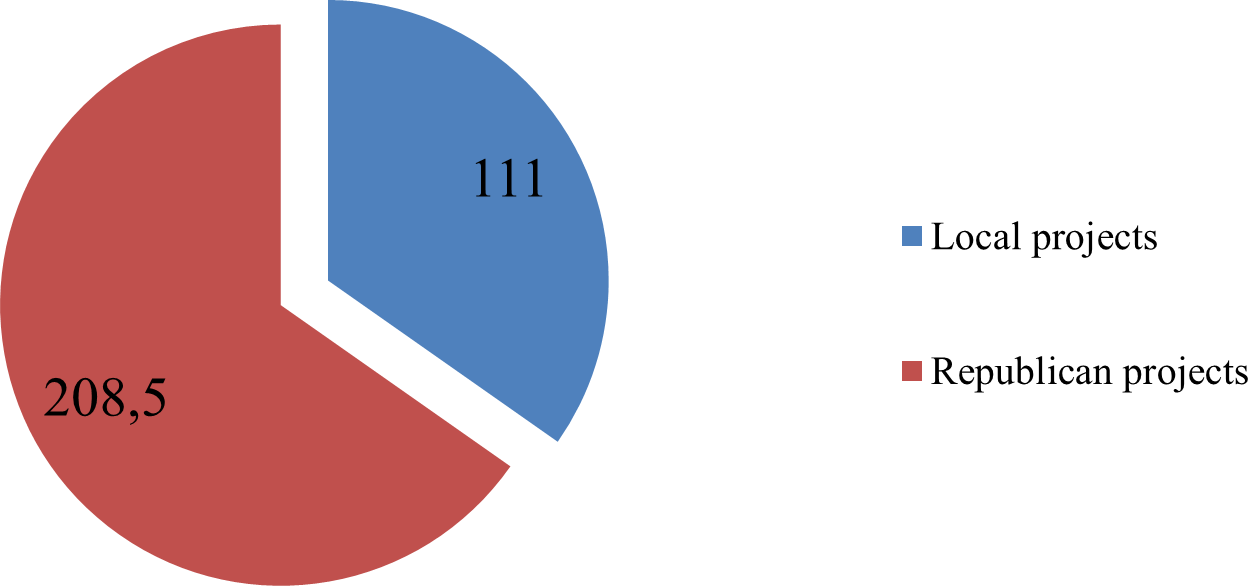
\includegraphics[width=0.55\textwidth]{media/ekon4/image19}
	\caption*{Fig.3 - Distribution of PPP projects by levels and government obligations, billion tenge}
	\caption*{\normalfont\emph{Note: Compiled by the author on the basis of data from JSC "Kazakhstan PPP Development Center" {[}6{]}}}
\end{figure}

\begin{multicols}{2}
According to the data provided, the largest number of government
commitment projects are in the East Kazakhstan region and the Turkestan
region. From the point of view of the state, the most capital-intensive
PPP projects are located in Astana and Atyrau region.

The figure below shows the distribution of PPP projects by levels and
government obligations, billion tenge. Fig.3

Of the 7 republican projects assessed, only one includes government
obligations in the amount of 208.5 billion tenge. The remaining 6
projects do not provide for direct obligations on the part of the state.
For PPP projects and local-level concessions, 66\% of government
obligations (73.3 billion tenge) fall on the following 9 projects. Table
3.
\end{multicols}

\tcap{Table 3 - Government obligations under PPPs and concessions at the local level (billion tenge)}
\begin{longtblr}[
  label = none,
  entry = none,
]{
  width = \linewidth,
  colspec = {Q[20]Q[619]Q[212]Q[71]},
  row{1} = {c},
  cell{2}{1} = {c},
  cell{2}{3} = {c},
  cell{2}{4} = {c},
  cell{3}{1} = {c},
  cell{3}{3} = {c},
  cell{3}{4} = {c},
  cell{4}{1} = {c},
  cell{4}{3} = {c},
  cell{4}{4} = {c},
  cell{5}{1} = {c},
  cell{5}{3} = {c},
  cell{5}{4} = {c},
  cell{6}{1} = {c},
  cell{6}{3} = {c},
  cell{6}{4} = {c},
  cell{7}{1} = {c},
  cell{7}{3} = {c},
  cell{7}{4} = {c},
  cell{8}{1} = {c},
  cell{8}{3} = {c},
  cell{8}{4} = {c},
  cell{9}{1} = {c},
  cell{9}{3} = {c},
  cell{9}{4} = {c},
  cell{10}{1} = {c},
  cell{10}{3} = {c},
  cell{10}{4} = {c},
  cell{11}{1} = {c=4}{0.942\linewidth},
  hlines,
  vlines,
}
№ & \textbf{Project			name} & \textbf{Place			of implementation} & \textbf{The			amount}\\
1 & Intelligent
			Traffic Safety and Analysis System (Sergec) & Almaty
			city & 14,2\\
2 & Landscaping
			of the territory of the city of Almaty & Almaty
			city & 8,1\\
3 & Organization
			of management of multifunctional complexes "Almaty - Arena"
			and "Halyk Arena" & {~\\~} & 5\\
4 & Current
			repair of the road network & Almaty
			city & 4,5\\
5 & Landscaping
			of Atyrau city & Atyrau
			city & 4,7\\
6 & Modernization
			and operation of canteens in 20 boarding schools & Turkestan
			region & 17,6\\
7 & Modernization
			and operation of canteens in the Centers for the provision of
			special social services to children with disabilities, the elderly
			and the disabled of groups I and II of the Office for the
			Coordination of Employment and Social Programs & Turkestan
			region & 6,5\\
8 & Organization
			and operation of children's and youth sports schools by sports & Turkestan
			region & 4,7\\
9 & Maintenance
			and maintenance of the B. Alexandrov Sports Palace & Ust-Kamenogorsk
			city & 8\\
Note:			Compiled by the author on the basis of the final report on the			evaluation of the implementation of PPP projects for 2023 of the			Kazakhstan Center for Public-Private Partnership [6] &  &  & 
\end{longtblr}

\begin{multicols}{2}
The most capital-intensive project with large private investments in the
creation (construction, reconstruction, overhaul) of a PPP facility at
the national level is the project "Providing broadband access to rural
settlements of the Republic of Kazakhstan using fiber-optic
communication lines technology", in which 74.6 billion tenge of private
funds have been invested. The second place in terms of private
investment is occupied by the republican PPP project "Implementation of
the horizontal monitoring platform" of the Ministry of Finance of the
Republic of Kazakhstan, with private investments in the amount of 10.0
billion tenge (the project is at the stage of termination of the PPP
agreement).

{\bfseries Results and discussion.} A public-private partnership is defined
as a contractual agreement between a public institution and a private
sector entity in which each sector shares skills, assets, risks, and
benefits in providing services or funds for use by the general public.
Public - private partnership has several advantages that can be noted:
private financing, as well as the rapid implementation of the approved
project, comprehensive implementation of public services, increasing the
risk to the business sector, as well as improving the efficiency of the
life cycle, etc. {[}8{]}.

Models of public-private partnership differ in each country, and its
effectiveness depends on the economic situation, legal framework,
institutional framework and historical structure. The article provides
several countries as examples, including countries such as Kyrgyzstan
and China.

So let' s move on to considering the PPP sector of
several countries in comparison. The models of Kyrgyzstan and Kazakhstan
in the field of PPP are similar to each other. However, there is a
difference and it depends on the level of institutional improvement and
the scale of implementation.

As for the Republic of Kazakhstan, the PPP system is developed here
thanks to the legislative framework, the creation of specialized
departments, as well as the implementation of large projects in the
transport, energy and social spheres.

And the number of such large projects in Kyrgyzstan is very small, and
there is not enough institutional support. In this country, the support
and development of the PPP system is now underway.

The economy of Kazakhstan is relatively stable and has a high potential
for entering the international market, which, in turn, will attract
foreign investment. And in Kyrgyzstan, economic and political
instability prevails, which is one of the high risks for investors.

In China, a system of public-private partnership is widely used in the
implementation of infrastructure projects. Chinese PPP models include:
see the table below (Table 4)
\end{multicols}

\tcap{Table 4 - Chinese PPP models}
\begin{longtblr}[
  label = none,
  entry = none,
]{
  width = \linewidth,
  colspec = {Q[185]Q[760]},
  row{1} = {c},
  cell{2}{1} = {c},
  cell{3}{1} = {c},
  cell{4}{1} = {c},
  cell{5}{1} = {c=2}{0.945\linewidth},
  hlines,
  vlines,
}
\textbf{Name} & \textbf{Definition}\\
Concessions: & Private
			companies receive the right to manage an infrastructure facility
			(such as a road or port) for a certain period of time, usually in
			exchange for payment through user fees.\\
Public-private
			agreements: & As
			part of the PPP, private companies participate in the design,
			construction or operation of facilities in partnership with the
			government. These agreements may include both partial and full
			private sector financing.\\
Concession
			agreements and state subsidies: & China
			often uses hybrid models where the private sector invests in
			projects, but the government also provides subsidies or
			guarantees.\\
Ke,			Y.J., Wang, S.Q. and Chan, A.P.C. (2009). “Public-Private			Partnerships in China’s Infrastructure Development: Lessons			Learnt.” Proceedings of Changing roles: new roles, new			challenges (CIB W096, W104), Noordwijk ann Zee, Netherlands,			October 5-9, 2009, 177-188 [9] & 
\end{longtblr}

\begin{multicols}{2}
In China, the main focus is on large-scale infrastructure projects, such
as the road industry, the construction of bridges, airports, as well as
housing construction. The country' s authorities manage
the risk by providing guarantees and support to private companies,
which, in turn, contributes to a decrease in the amount of losses.

All the processes that the state is doing in the direction of PPP are
associated with preventing the project from becoming unprofitable for
the state.

The Chinese authorities understand that PPP is not a universal solution.
That is, it takes into account that it is a tool that is used to its
advantage, taking into account all the risks and benefits that may occur
{[}9{]}

China is one of the most steadily developing countries. The need for
infrastructure is at a high level, which puts pressure on the budget of
the Chinese country. Private investors cannot afford to master the size
of the Chinese infrastructure market. Entrepreneurship is interested in
the PPP sector, and the public sector' s interest in
increasing efficiency through private investment contributes to making
the best decisions on the development of PPP.

China has been found to have a wealth of experience with PPP, and the
number of PPP projects will continue to grow in the future. However, an
insufficiently developed institutional and regulatory framework does not
guarantee the sustainability of PPP projects. Investors should align
their interests with the public sector and therefore receive support
from local authorities, especially for projects with a weak ability to
generate income {[}10{]}.

In Australia, PPP is also widely used, especially in the construction
and maintenance of infrastructure. Main features: see table 5.
\end{multicols}

\tcap{Table 5 - PPP models used in Australia}
\begin{longtblr}[
  label = none,
  entry = none,
]{
  width = \linewidth,
  colspec = {Q[175]Q[767]},
  row{1} = {c},
  cell{2}{1} = {c},
  cell{3}{1} = {c},
  cell{4}{1} = {c=2}{0.942\linewidth},
  hlines,
  vlines,
}
\textbf{Name} & \textbf{Definition}\\
Models
			with variable risk: & In
			Australia, there is a practice of distributing risks based on the
			parties' ability to cope with them. For example, construction
			risks may be borne by the private sector, while operational risks
			may remain at the government level.\\
Public-private
			agreements and concessions: & Australia
			actively uses the concession model, where the private sector gets
			the right to manage infrastructure, but in the case of social or
			strategically important facilities, private participation is
			limited.\\
Australian			Government Department of Infrastructure, Transport, Regional			Development and Communications\textbf{.			}(2022).			Public-Private Partnerships: A Guide to Best Practice [11] & 
\end{longtblr}

\begin{multicols}{2}
In Australia, PPP finds a balance between private and public
participation, with an emphasis on long-term efficiency and strategic
planning.

In Kazakhstan, there is a dynamic development of public private
partnership (PPP), while a variety of models are used in the market: see
table 6.
\end{multicols}

\tcap{Table 6 - PPP models used in Kazakhstan}
\begin{longtblr}[
  label = none,
  entry = none,
]{
  width = \linewidth,
  colspec = {Q[198]Q[746]},
  row{1} = {c},
  cell{2}{1} = {c},
  cell{3}{1} = {c},
  cell{4}{1} = {c},
  cell{5}{1} = {c=2}{0.944\linewidth},
  hlines,
  vlines,
}
\textbf{Name} & \textbf{Definition}\\
Government
			guarantees: & As
			part of the PPP, the government provides guarantees to private
			companies that reduce the risks associated with possible changes
			in the economic situation.\\
Concessions
			and partially private projects: & There
			are projects where private investors can build and operate
			infrastructure, but critical functions such as providing social
			services or regulating tariffs remain under government control.\\
{
			Models
			with partial private sector financing:
			\\~\\~} & {
			Kazakhstan
			actively attracts private investment through co-financing
			mechanisms. In such projects, the government and the private
			sector share the risks and benefits.
			\\~\\~}\\
Compiled			by the author on the basis of a scientific article by			Soltangazinov A.R., Isenova G.K., Kaidarova L.K. Models and forms			of public–private partnership, Bulletin of the Belgrade			University of Cooperation, Economics and Law			[12] & 
\end{longtblr}

\begin{multicols}{2}
Public-private partnership (PPP) is an important tool for solving public
problems and infrastructure development in Kazakhstan. Taking into
account the current development process, the variety of problems
encountered, we believe that digitalization of public-private
partnership should be a factor in the successful completion of projects
today.

The introduction of digital technologies in the sphere of public-private
partnership will increase the efficiency of the state and business, as
well as improve the quality of public services, reduce costs associated
with money transfers and ensure transparency of all ongoing activities.
\end{multicols}

\tcap{Table 7 - Common international PPP models}
\begin{longtblr}[
  label = none,
  entry = none,
]{
  width = \linewidth,
  colspec = {Q[44]Q[90]Q[425]Q[383]},
  rows = {font = \scriptsize},
  cell{6}{1} = {c=4}{0.942\linewidth},
  hlines,
  vlines,
}
\textbf{№} & \textbf{Analyzed countries} & \textbf{PPP Models} & \textbf{Institutional and legal features}\\
1 & Kazakhstan & {Active implementation of PPPs since the early 2000s.\\\\Concession and joint investment projects prevail.\\\\The government is actively involved in attracting foreign investors.\\\\Main areas: transport, energy, Housing and communal services.\\\\Implementation of specialized legislation on PPP.} & {Special government agencies and agencies for the development of PPPs have been created.\\\\Legislation is constantly being improved.\\\\The legal framework is well-established.\\\\The institutional infrastructure is developing, which makes it possible to gradually reduce risks and increase transparency.}\\
2 & Kyrgyzstan & {The PPP model is developing gradually, and concession and lease schemes are often used.\\\\The main focus is on socially significant objects (roads, communal infrastructure).\\\\Problems: limited private capital, lack of an institutional base.} & {The insufficiently developed legislative framework governing PPPs.\\\\Lack of clear support mechanisms and guarantees for private investors.\\\\The institutional structures responsible for PPPs operate with limited resources and low coordination.\\\\International financial organizations that provide technical and financial assistance play an important role.}\\
3 & China & {China is actively using PPP in infrastructure projects such as the construction of transport networks and energy generation.\\\\The main model is a concessional one, often with elements of co—financing.\\\\PPPs in China have strict regulation and government support, which makes it possible to scale projects quickly.\\\\The focus is on large infrastructure projects involving public and private companies.} & {A comprehensive regulatory framework has been formed to regulate various types of PPPs.\\\\The system of public-private interaction is highly institutionalized.\\\\Strong administrative resources and centralized control contribute to the rapid scaling of projects.\\\\The private sector is actively involved, but subject to clear government frameworks and constraints.}\\
4 & Australia & {One of the most developed and mature PPP systems.\\\\A variety of forms are used, from concessions to long—term contracts.\\\\Emphasis on efficiency and transparency, extensive experience in attracting private investment in social and transport infrastructure.\\\\Clear legislation and well - developed institutional infrastructure} & {A clear and well-developed legislative framework governing all aspects of PPPs.\\\\Availability of specialized agencies and bodies responsible for project support.\\\\A high level of institutional maturity, which allows effective risk management and ensuring a balance of interests.\\\\Public audit and reporting systems promote high transparency and trust on the part of investors and society.}\\
Note: the analysis is based on sources [6 , 8, 9]. &  &  & 
\end{longtblr}

\begin{multicols}{2}
The success of PPP models depends on a balance between active government
support, a developed and transparent legal framework, and a mature
institutional infrastructure capable of effectively managing projects
and risks.

- In developed countries such as Australia, high institutional maturity
and legal transparency create comfortable conditions for private
investors and society.

- In countries with economies in transition (Kazakhstan, Kyrgyzstan), it
is important to work on improving the legislative framework and
developing PPP institutions.

- China is showing an example of strong government regulation and
centralized project management, which allows for the rapid
implementation of large-scale initiatives.

Thus, the international experience of PPP shows that the success of the
model depends on a balance of government support, a developed legal
framework, the ability of the private sector and the priority of
strategically important industries for the country.

In the Republic of Kazakhstan, in recent years, the process of
digitalization of the PPP industry has been carried out on a large
scale. It is considered very useful for the following aspects:

Project management: you can improve the efficiency and accuracy of
decision-making by using digital tools to track and evaluate the
implementation of PPP projects.

Modern information devices can combine information about the risks
associated with the project, deadlines and costs associated with it,
which allows you to effectively evaluate and manage projects in real
time.

List of anti-corruption measures: digitalization of the process reduces
the possibility of the human factor, which, in turn, increases
transparency in the implementation of the PPP project and reduces the
possibility of corruption. Allows you to increase the transparency of
online reporting platforms and electronic tender procedures.

The joint work of the state and entrepreneurship will allow: to improve
the use of digital platforms for the exchange of information between
government agencies and private companies, reduce paperwork and reduce
the stages of concluding contracts.

Sustainability and adaptability: digitalization of the PPP industry
increases its ability to quickly adapt to changes in the external
environment. Software solutions based on big data and artificial
intelligence can predict potential problems in advance and suggest ways
to solve it.

The Republic of Kazakhstan has been actively introducing digital
technologies into the PPP industry in recent years. As a great example,
I can mention the public procurement portal, which is a platform that
contributes to open access to Information, selection of contractors on
the most objective basis. Details can be found below (Table.7)
\end{multicols}

\tcap{Table 8 -- Digital projects and platforms operating in the Republic of Kazakhstan for 2024}
\begin{longtblr}[
  label = none,
  entry = none,
]{
  width = \linewidth,
  colspec = {Q[183]Q[679]Q[81]},
  cell{1}{1} = {c},
  cell{1}{2} = {c=2}{0.758\linewidth},
  cell{2}{1} = {c},
  cell{2}{3} = {c},
  cell{3}{1} = {c},
  cell{3}{3} = {c},
  cell{4}{1} = {c},
  cell{4}{3} = {c},
  cell{5}{1} = {c},
  cell{5}{3} = {c},
  cell{6}{1} = {c},
  cell{6}{3} = {c},
  cell{7}{1} = {c},
  cell{7}{3} = {c},
  cell{8}{1} = {c=3}{0.943\linewidth},
  hlines,
  vlines,
}
\textbf{Name of the platform/project} & \textbf{Purpose, and Year of activation} &\\
Public Procurement Portal & the
			main electronic resource for conducting tenders and contests,
			which ensures transparency and accessibility of information on
			public procurement. This portal is used to electronically place
			orders, participate in tenders, and monitor the execution of
			contracts. & 2006\\
Electronic Monitoring and Management System for PPP Projects (e-Gov) & This
			system allows you to effectively monitor the progress of PPP
			projects in real time, which contributes to a more timely response
			to emerging problems and deviations from schedule. & 2004\\
Smart Government Monitoring system & This
			system is used to analyze and predict risks in PPP projects, as
			well as to assess their financial and technical effectiveness. It
			collects information and processes it at regular intervals. In
			turn, this contributes to the rapid and effective decision-making
			of government agencies. & 2017-2018\\
Public
			procurement platform of the Republic of Kazakhstan & A
			system for improving the transparency and efficiency of the public
			procurement process using digital technologies aimed at automating
			the procedures for submitting applications and evaluating
			proposals. & 2017\\
Integrated
			electronic procurement system & An
			e-procurement platform that ensures the mutually beneficial work
			of the state and entrepreneurship, as well as transparency in the
			process of conducting tenders. & 2019\\
PPP
			digital information system of the Republic of Kazakhstan & This
			project will allow you to carry out control work at all stages of
			the implementation of PPP projects and provide all interested
			parties with reliable information in a timely manner. & 2020\\
Note:
			the table was compiled by the author based on the analysis of
			domestic digital platforms in the field of PPP. &  & 
\end{longtblr}

\begin{multicols}{2}
State bodies are actively implementing digital technologies in order to
control the work of public-private partnership. An important step was
also the development of infrastructure for data collection and
processing, which contributes to a more accurate analysis of the state
of affairs and risk forecasting.

Despite the obvious advantages, the digitalization of the PPP system in
Kazakhstan faces a number of challenges:

Technical and organizational barriers: Not all public and private
institutions are ready to fully integrate digital solutions, which can
slow down the digitalization process.

Lack of standards and protocols for data exchange: Kazakhstan does not
yet have uniform standards for working with digital data, which leads to
difficulties in integrating various information systems.

Cybersecurity: The introduction of digital solutions increases the risks
of cyber attacks, which requires the government and private companies to
take additional measures to protect information.

A number of measures must be taken to successfully digitalize the PPP
system in Kazakhstan.:

Development of a unified platform for managing PPP projects, which will
ensure transparency, convenience and the possibility of integration with
other government systems.

Creation of standards and protocols for data exchange, which will
improve interaction between various PPP participants.

Professional development of civil servants and private sector
specialists in the field of digital technologies, which will ensure more
efficient use of digital solutions.

Strengthening cybersecurity at all levels of implementation of PPP
projects in order to protect data and prevent possible threats.

Digitalization is a significant factor contributing to the development
of the public-private partnership system in Kazakhstan. The introduction
of digital technologies in project management processes contributes to
improving the transparency and efficiency of interaction between public
and private organizations. However, to achieve a fully digitized system,
it is necessary to develop a single infrastructure, standards.
Strengthening cybersecurity measures is also considered important
{[}13{]}.
\end{multicols}

\tcap{Table 9 - SWOT analysis of the state of Public-Private Partnership in the Republic of Kazakhstan}
\begin{longtblr}[
  label = none,
  entry = none,
]{
  width = \linewidth,
  colspec = {Q[502]Q[442]},
  row{1} = {c},
  row{3} = {c},
  cell{5}{1} = {c=2}{0.944\linewidth},
  hlines,
  vlines,
}
Strengths & Weaknesses\\
{State support\\\\Growth of private investment\\\\Implementation of a diverse project in a short time\\\\Digitalization of processes\\\\Contributing to the development of the private sector} & {Technical and organizational barriers\\\\Legislative acts still need to be developed\\\\Dependence on public funding\\\\Challenges in project management at the local level}\\
Opportunities & Danger\\
{Expanding digital platforms and integrating solutions\\\\International cooperation and attracting foreign investment\\\\Smart cities and environmental projects\\\\Support and development of entrepreneurship through PPP\\\\Using artificial intelligence and big data} & {Economic instability and external risks\\\\Political risks and legislative changes\\\\Cyber threats and data security\\\\Bureaucracy and administrative barriers\\\\Uncertainty in project deadlines and budgets}\\
Note: the table was compiled by the author based on the analysis of the data presented in the scientific work. & 
\end{longtblr}

\begin{multicols}{2}
The results of the SWOT analysis. It showed a significant development in
the development of public-private partnership in Kazakhstan. This is
primarily due to the increase in state support for the introduction of
digital technologies and the attraction of private investment. However,
it was noted that the current system faces a number of obstacles,
including such problems as lack of standards, organizational
difficulties and dependence on foreign economic factors. Eliminating
these weaknesses, effective use of digitalization and opportunities for
international cooperation can significantly increase the profitability
and sustainability of PPP projects in Kazakhstan.

{\bfseries Conclusion}. In recent years, the PPP mechanism in the Republic
of Kazakhstan has become an important tool for modernizing
infrastructure and social spheres. Owl is actively using this tool in
the direction of attracting private investment.

Digitalization of PPP projects is becoming a key factor in improving
their efficiency and sustainability. The introduction of modern
information systems contributes to improving the quality of project
management, ensuring transparency of processes, accelerating them and
reducing corruption risks. The first results in this direction are
assessed positively, although the need to improve the system is still
relevant.

At the same time, a number of serious problems arise in the process of
digitalization. In particular, the lack of uniform data exchange
standards, technical and organizational restrictions, as well as risks
in the field of cybersecurity hinder the full implementation of digital
technologies in the PPP system.

To fully realize the digital potential, it is recommended to implement
the following measures:

- creation of a single digital platform for managing PPP projects, which
will effectively coordinate all stages of the system;

- development of standardized data exchange protocols, necessary to
ensure effective integration between all stakeholders;

- strengthening cybersecurity, increasing the level of protection of
data and systems;

- systematic professional development of specialists, development of
training programs and professional development courses;

- improvement of incentive measures for private investors, including the
formation of a system of financial benefits and guarantees;

- support for the introduction of innovative technologies, which will
improve the quality and efficiency of PPP projects.

The mechanism of public-private partnership in Kazakhstan serves as an
important tool in modernizing infrastructure, improving the quality of
social services and attracting private investment.In recent years, the
digitalization process has been prioritized in this area, which in turn
contributes to increasing the transparency of projects, reducing
corruption risks and improving interaction between government agencies
and the private sector.

The introduction of modern digital technologies in the PPP project
management process will improve the quality of control and monitoring,
timely focus on risks and optimize management processes. Electronic
equations, automated project tracking and management systems, as well as
updated data standards are aimed at ensuring the efficiency and
sustainability of the implementation of infrastructure projects.

However, there are also problems that need to be solved in order to
fully realize this potential. In particular, barriers of a technical and
organizational nature, the lack of uniform data exchange standards and
threats to cybersecurity remain as the main factors hindering digital
transformation. Therefore, the systematic solution of these difficulties
will become a prerequisite for the effective implementation of
digitalization and the high-quality development of PPP projects.

It is important to develop a single digital platform for managing
public-private partnership projects that will ensure effective work
between all participants, as well as develop data standards to simplify
the workflow and ensure transparency. It is also worth paying attention
to the issue of advanced training of specialists in the field of digital
technologies. This will help introduce digital solutions to PPP models
and concessions, accelerate their development and strengthen interaction
between the state and entrepreneurship.

The introduction of blockchain-based smart contracts will improve the
efficiency and transparency of public-private partnership agreements
through electronic transactions. {[}4{]}. In addition, integrating big
information analytics into decision-making methods allows you to
optimize resource allocation and project development. {[}3{]}. Creating
a reliable and effective regulatory framework and a convenient legal
framework is very important for digital PPP in a safe and innovation --
friendly environment. {[}2{]}. As a result of successful digitalization,
the PPP system in Kazakhstan will not only be able to effectively solve
the problems of social and infrastructural modernization, but also
become an important tool for sustainable economic growth, as well as
improving the quality of life of citizens.

Future research should evaluate digital PPP applications across sectors
and compare global best practices. Focus areas include regulatory
changes, cybersecurity and AI-driven governance {[}14{]}. Effective
digitalization will ensure PPPs contribute to sustainable economic
growth and better public services.
\end{multicols}

\begin{center}
{\bfseries Литература}
\end{center}

\begin{references}
1. Poslanija Prezidenta narodu Kazahstana za 2020-2024 gg.
\href{https://www.akorda.kz/ru/addresses}{https://www.akorda.kz} .- Data obrashhenija: 04.01.2025.{[}in
Russian{]}

2. Ismailova R.A., Zhandaulet B. Analiz primenenija i perspektivy
razvitija gosudarstvenno chastnogo partnerstva v Respublike Kazahstan.
-2023. ‒ №2 (51).- C.91-100. DOI \\10.52260/2304-7216.2023.2(51) .12. {[}in
Russian{]}

3. Ajtkalieva A.M., Galieva A.H., Toksanova A.N. Razvitie gosudarstvenno
chastnogo partnerstva v transp\-ortnoj infrastrukture Respubliki
Kazahstan//Jekonomicheskaja serija vestnika ENU imeni L.N. Gumileva.
-2022. -№1. - S.19-31. DOI 10.32523/2789-4320-2022-1-19-31.{[}in
Russian{]}

4. Lukpanova Zh.O, TyngishevaA.M.,Napravlenija razvitija gosudarstvenno
chastnogo partnerstva v zdra\-voohronenii Kazahstana // VESTNIK Kazahskogo
universiteta jekonomiki, finansov i mezhdunarodnoj torgovli, 2022 - №4
(49) VESTNIK Kazahskogo universiteta jekonomiki, finansov i
mezhdunarodnoj torgovli. - 2022 - №4 (49) DOI
10.52260/2304-7216.2022.4(49).28.{[}in Russian{]}

5. Asian Development bank: «Obzor gosudarstvenno -- chastnogo
partnerstva Kazahstan»

6. Oficial' nyj sajt AO «Kazahstanskij centr razvitija
GChP» \href{https://ppp-center.kz/}{https://ppp-center.kz} .-Data obrashhenija: 04.01.2025. {[}in
Russian{]}

7. Nacional' naja palata predprinimatelej RK «Atameken»
Gosudarstvenno-chastnoe partnerstvo\\
\href{https://atameken.kz/ru/services/18-gosudarstvenno-chastnoe-partnerstvo}{https://atameken.kz} .- Data
obrashhenija: 04.01.2025.{[}in Russian{]}

8. Chan A.P.C., Lam P.T.I., Chan D.W.M., Cheung E. and Ke Y.J. Drivers
for Adopting Public Private Partnerships -- Empirical Comparison between
China and Hong Kong Special Administrative Region// Journal of
Construction Engineering and Management.-2009.- Vol.135(11).-
P.1115-1124. DOI\\
\href{http://dx.doi.org/10.1061/(ASCE)CO.1943-7862.0000088}{10.1061/(ASCE)CO.1943-7862.0000088}

9. Ke Y.J., Wang S.Q. and Chan A.P.C. ``Public-Private Partnerships in
China's Infrastructure Development: Lessons Learnt.'' Proceedings of
Changing roles: new roles, new challenges (CIB W096, W104), Noordwijk
ann Zee, Netherlands, October 5-9, 2009, 177-188.
\href{https://www.researchgate.net/publication}{https://www.researchgate.net} .- Date of address:\\
04.01.2025.

10. Ke Y., Jefferies M., Shrestha A., Jin X. Public Private Partnership
in China: Where to from Here // Organization, Technology \& Management in
Construction.-2014.-Vol/6(3).-P.1156-1162. DOI\\
\href{http://dx.doi.org/10.5592/otmcj.2014.3.10}{10.5592/otmcj.2014.3.10}

11. Australian Government Department of Infrastructure, Transport,
Regional Development and Commun\-ications. (2022). Public-Private
Partnerships: A Guide to Best Practice.
\href{https://www.infrastructure.gov.au/infrastructure-transport}{https://www.infrastructure.gov.au} .- Date of address:04.01.2025.

12. Солтангазинов А.Р., Исенова Г.К.,Кайдарова Л.К. Модели и формы
государственно -- частного партнерства//Вестник Белградского
университета кооперации, экономики и права. -2019. -№5 (78).- С.95-104.
DOI 10.21295/2223-5639-2019-5-95-104

13. \href{https://primeminister.kz/ru}{Официальный информационный ресурс
Премьер-министра Республики Казахстан} Автоматизированы 82\% госуслуг и
оказано более 54 млн услуг в электронном формате --- итоги цифрового
развития. \href{https://primeminister.kz/ru/news}{https://primeminister.kz} .- Дата
обращения 04.01.2025

14. Yermekbayev, A., et al. (2022). Opportunities and prospects of
public-private partnership for technolog\-ical development of mining and
metallurgical complex enterprises of Kazakhstan// Bulletin of the
Karag\-anda University: Economy Series .- 2022.- Vol.102(4).-
P.89-104. DOI 10.31489/2022ec3/34-44
\end{references}

\begin{authorinfo}
\emph{{\bfseries Информация об авторах}}

Жумажанова М.Т.- старший преподаватель, магистр, АО «Казахский
университет технологии и бизнеса им. К. Кулажанова», Астана, Казахстан
e-mail: maral2804@mail.ru;

Сапарова Б.С.- к.э.н., профессор «Евразийский национальный университет
имени Л.Н.Гумилева» Астана, Казахстан. e-mail: sbsfmenu@mail.ru;

Syed Faisal Hassan Bukhari- PhD, профессор, Воздушный университет,
Исламабад, Пакистан e-mail: \\nadealishanawer@gmail.com

\emph{{\bfseries Information about the authors}}

Zhumazhanova M.- Senior Lecturer, Master's Degree, «Kazakh University of
Technology and Business named after K. \\Kulzhanov», Astana, Kazakhstan,
e-mail: maral2804@mail.ru;

Saparova B.- Candidate of Economics, Professor, L.N.Gumilyov Eurasian
National University, Astana, Kazakhstan, e-mail: sbsfmenu@mail.ru;

Syed Faisal Hassan Bukhari - PhD Professor, Air University, Islamabad,
Pakistan. e-mail: nadealishanawer@gmail.com.
\end{authorinfo}
